%%%%%%%%%%%%%%%%%%%%%%%%%%%%%%%%%%%%%%%%%%%%%%%%%%%%%%%%%%%%%%%%%%%%%%
% Problem statement
\begin{statement}[
  problempoints=70,
  timelimit=1 second,
  memorylimit=512 MiB,
]{Slagalica}

Little Fabian got a one-dimensional jigsaw puzzle that consists of $N$ pieces.
He quickly realized that each piece belongs to one of the following types:\\

\begin{figure}[H]
\centering
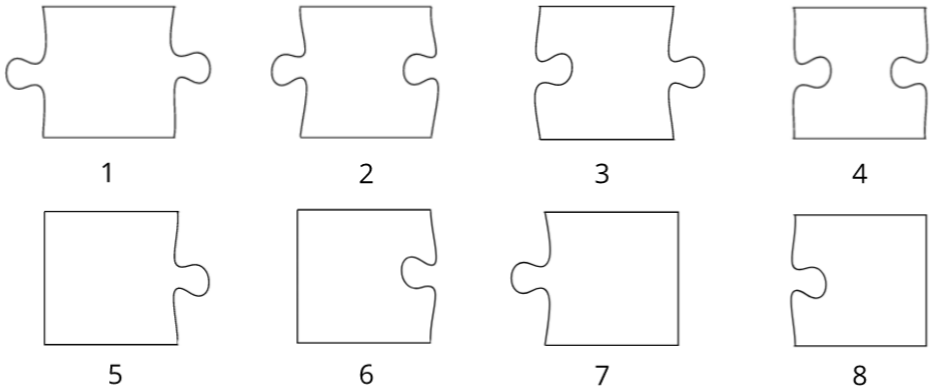
\includegraphics[width=0.6\textwidth]{img/puzzledef.png}
\end{figure}

Additionally, it is known that among those $N$ pieces there is exactly one piece
of either type $5$ or type $6$ (left border) and exactly one piece of either type
$7$ or type $8$ (right border).

Fabian wishes to arrange all of the pieces into a single row such that
the first (leftmost) piece is of type $5$ or $6$ and the last (rightmost) piece
is of type $7$ or $8$. Two pieces can be placed next to each other if and only
if their neighbouring borders are of different shapes, i.e., one has a bump
(also called \textit{outie} or \textit{tab}) and the other has a hole (also
called \textit{innie} or \textit{blank}).

Simply solving the puzzle would be too easy for Fabian so he decided to write
a unique positive integer on each of the pieces. Now he is interested in finding
the lexicographically smallest solution to the jigsaw puzzle. The solution $A$
is considered lexicographically smaller than solution $B$ if at the first
position (from the left) $i$ where they differ it holds that the number written
on $i$-th puzzle in $A$ is smaller than the number written on $i$-th puzzle in
$B$.

\textbf{Note:} the pieces cannot be rotated.

%%%%%%%%%%%%%%%%%%%%%%%%%%%%%%%%%%%%%%%%%%%%%%%%%%%%%%%%%%%%%%%%%%%%%%
% Input
\subsection*{Input}
The first line contains an integer $N$ $(2 \le N \le 10^5)$ from the task
description.

The next $N$ lines contain two integers $X_i$ $(1 \le X_i \le 8)$ and $A_i$
$(1 \le A_i \le 10^9)$ which represent the type of the $i$-th piece and the
number Fabian wrote on it. All numbers $A_i$ will be different.

%%%%%%%%%%%%%%%%%%%%%%%%%%%%%%%%%%%%%%%%%%%%%%%%%%%%%%%%%%%%%%%%%%%%%%
% Output
\subsection*{Output}
If Fabian cannot solve the jigsaw puzzle, you should output $-1$ in a single
line.

Otherwise, you should output the numbers that are written on the pieces in the
lexicographically smallest solution to the puzzle.

%%%%%%%%%%%%%%%%%%%%%%%%%%%%%%%%%%%%%%%%%%%%%%%%%%%%%%%%%%%%%%%%%%%%%%
% Scoring
\subsection*{Scoring}
In test cases worth a total of $5$ points it will hold $N \le 4$.\\
In test cases worth additional $5$ points it will hold $N \le 10$.\\
In test cases worth additional $10$ points pieces of types $2$ and $3$ will not
                                            appear in the input.\\
In test cases worth additional $20$ points there will be at most one piece of
                                           type $1$ or $4$.

If for some test case in which the solution to the puzzle exists, you output the
correctly solved puzzle but your solution is not lexicographically smallest, you
will get $40\%$ of the points intended for that test case.

%%%%%%%%%%%%%%%%%%%%%%%%%%%%%%%%%%%%%%%%%%%%%%%%%%%%%%%%%%%%%%%%%%%%%%
\subsection*{Examples}
\begin{tabularx}{\textwidth}{X'X'X}
\sampleinputs{test/slagalica.dummy.in.1}{test/slagalica.dummy.out.1} &
\sampleinputs{test/slagalica.dummy.in.2}{test/slagalica.dummy.out.2} &
\sampleinputs{test/slagalica.dummy.in.3}{test/slagalica.dummy.out.3}
\end{tabularx}

\textbf{Clarification of the first example:}\\
There are only two possible solutions to the puzzle:\\

\begin{figure}[H]
\centering
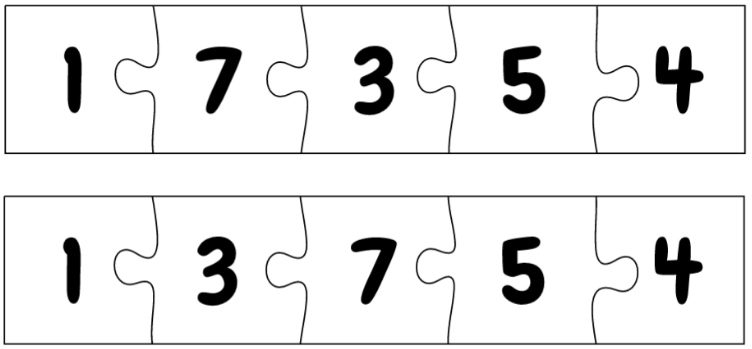
\includegraphics[width=0.6\textwidth]{img/sample_clarification.png}
\end{figure}
We can see that the second depicted solution has a smaller number written
on the second piece. Therefore, that is the lexicographically smallest solution.

%%%%%%%%%%%%%%%%%%%%%%%%%%%%%%%%%%%%%%%%%%%%%%%%%%%%%%%%%%%%%%%%%%%%%%
% We're done
\end{statement}

%%% Local Variables:
%%% mode: latex
%%% mode: flyspell
%%% ispell-local-dictionary: "croatian"
%%% TeX-master: "../hio.tex"
%%% End:
